%/*******************************************************************************
% * Copyright (c) 2007-2010, G. Weirich
% * All rights reserved. This program may not be distributed
% * or modified without prior written consent
% *
% * Contributors:
% *    G. Weirich - initial implementation
% *    T. Schaller - Physiotherapie
% *
% *  $Id: elexis-arzttarife-schweiz.tex 5164 2009-02-21 10:45:40Z rgw_ch $
% *******************************************************************************/
\documentclass[a4paper]{scrartcl}
\usepackage{german}
\usepackage[utf8]{inputenc}
\usepackage{makeidx}
\usepackage{wrapfig}
\makeindex

\usepackage[pdftex]{graphicx}
\DeclareGraphicsExtensions{.pdf,.jpg,.png}

\usepackage{floatflt}
\usepackage[]{hyperref}
\usepackage{color}
\title{Abrechnen mit Tarmed \& Co.}
\author{Gerry Weirich}

\begin{document}

\extratitle{
    \vfill
	\begin{center}
		
\includegraphics{tarmedbuch2}
	\end{center}

%    \begin{center}
%    Handbuch für die Abrechnung nach Tarmed
%    \end{center}
%    \vfill
   \begin{center}
  \copyright 2008-2010 by G.Weirich. Nachdruck und Weitergabe, auch auszugsweise, sowohl in elektronischer als auch in Papierform, nur mit Genehmigung des Autors.

    \end{center}
    \vfill
}
\maketitle

\tableofcontents
\clearpage
\section{Einführung}
Der Weg vom Erbringen einer Leistung bis zum Einbuchen der Zahlung umfasst eine ganze Reihe verschiedener Schritte, die korrekt aufeinander abgestimmt werden müssen. Diese Broschüre erklärt die Konzepte und das Vorgehen beim Tarmed-System.

\bigskip

\begin{picture}(200,10)
\line(100,0){200}
\end{picture}

\textbf{Achtung:} Es kann nicht garantiert werden, dass alle in dieser Broschüre gemachten Angaben richtig sind und zu korrekten Rechnungen führen. Für die Korrektheit der von Ihnen erstellten Rechnungen sind in erster Linie Sie selber verantwortlich. Es wird daher dringend empfohlen, dass Sie Ihre Rechnungen vor dem Versand kontrollieren.

\begin{picture}(200,10)
\line(100,0){200}
\end{picture}

\bigskip

Folgende Fragen müssen beantwortet werden, um korrekte Rechnungen zu erstellen und Zahlungen entgegenzunehmen\footnote{Dies ist nicht Elexis-spezifisch, sondern muss in jedem Praxisprogramm 'irgendwie' festgelegt werden. Bloss kann es bei weniger flexiblen Programmen 'festverdrahtet' sein, oder bei manchen Installationsverträgen kann die Konfiguration schon vom Hersteller vorgenommen werden sein. Da Elexis aber 'empowerment' des Anwenders auf den Fahnen stehen hat, müssen und dürfen Sie diese Dinge hier selber in die Hand nehmen (oder sich selber eine Supportfirma suchen, die es für Sie macht).}:

\begin{itemize}
\item Welches Tarifsystem und welche Tarifstufe wende ich an?
\item Für wen rechne ich ab?
\item An wen geht die Rechnung (und in welcher Form geht sie dorthin)?
\item Wer ist Kostenträger?
\item Wie identifiziere ich meine Leistungen gegenüber dem Kostenträger?
\item wohin sollen die Zahlungen gehen?
\item Woher weiss ich, ob Zahlungen eingegangen sind?
\item Wann und wie mahne ich?
\item Wann und wie leite ich Betreibungen ein?
\end{itemize}

Im Folgenden werde ich diese Schritte einzeln zeigen und die entsprechenden notwendigen Konfigurationen darlegen.

\section{Schritt für Schritt: Konfiguration}
Es sei an dieser Stelle nochmal darauf hingewiesen, dass diese Konfiguration nicht ganz trivial ist. Im Zweifelsfall sollten Sie es von einem Supporter durchführen lassen und stattdessen gleich im Abschnitt \ref{rechnungenerstellen} auf Seite \pageref{rechnungenerstellen} weiterlesen.

\medskip

\subsection{Abrechnungssysteme}
\label{Abrechnungssysteme}
\index{Abrechnungssystem}\index{UVG}\index{KVG}\index{VVG}\index{Privatrechnung}\index{Physiotherapie}
Die Leistungsverrechnung ist in Elexis als Plugin realisiert und damit auswechselbar oder auch ergänzbar - man kann nach Tarmed und nach CHOP, nach einem beliebigen Privatrechnungssystem und/oder nach einem österreichischen System abrechnen, das hängt nur davon ab, welche Plugins man installiert hat. Auch der Wechsel auf ein jetzt noch nicht bekanntes Tarifsystem ist damit kein Problem. Jedes Tarif-Plugin enthält das Codesystem selbst, sowie einen Mechanismus, um Rechnungen auszugeben, die zu diesem System konform sind (so muss eine Tarmed-Rechnung nicht nur andere Positionen beinhalten, sondern auch formal anders aussehen, als etwa eine Privatrechnung einer Heilpraktikerin). Ausserdem beinhaltet ein Abrechnungssystem je nachdem bestimmte Angaben, die vorhanden sein müssen, um Rechnungen erstellen zu können (z.B. Kostenträger, Versicherungsnummer u. Ä.)


\medskip

\index{Leistungscode}
Leistungscode, Ausgabeziel und erforderliche Daten, sowie die Tarifstufe sind in Elexis als 'Abrechnungssystem' zusammengefasst (S. Abb. \ref{fig:abr1}):
\begin{figure}
  % Requires \usepackage{graphicx}
  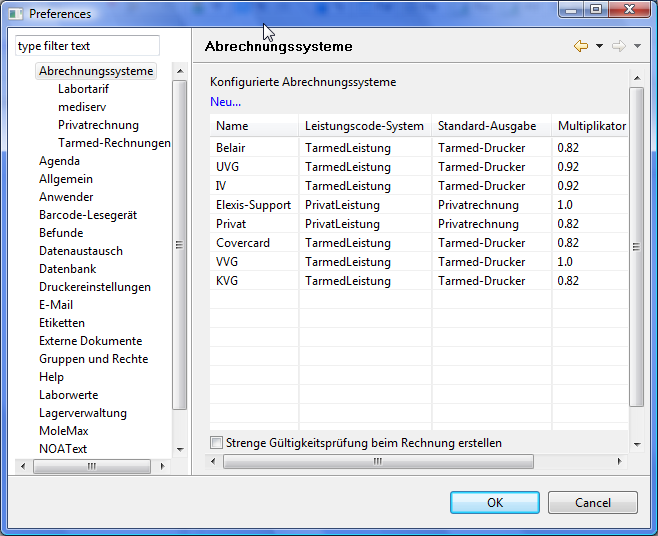
\includegraphics[width=0.9\textwidth]{abr1}\\
  \caption{Abrechnungssysteme: Übersicht}\label{fig:abr1}
\end{figure}
Es kann beliebig viele Abrechnungssysteme geben, und die Namen der einzelnen Abrechnungssysteme sind seitens Elexis egal. Um alle Schweizer Systeme abzudecken, sollten allerdings Abrechnungssysteme mit den Namen 'KVG', 'UVG', 'IV', 'MV' und 'VVG' vorhanden sein. Weitere können nach Belieben dazukommen. Es ist beispielsweise problemlos möglich, zwei verschiedene KVG-Systeme mit verschiedenen Taxpunktwerten zu definieren. Wenn das Plugin elexis-arzttarife-schweiz installiert ist (standardmässig ist das bei in der Schweiz installierten Elexis-Systemen immer der Fall), dann sind die Leistungscodes Tarmed, Analysenliste und Physiotherapietarif bereits eingeschlossen und die oben erwähnten Standard-Abrechnungssysteme werden beim ersten Erstellen eines Falls automatisch angelegt. Bei einer ganz frischen Elexis-Installation sollten Sie daher zunächst einen Patienten und einen Fall erstellen, um das Leistungscode-System zu initialisieren, damit Sie das nicht manuell machen müssen.

\medskip

Um ein neues Abrechnungssystem zu erstellen, klickt man auf 'Neu...', um ein bestehendes zu modifizieren, klickt man doppelt darauf. Es öffnet sich der Abrechnungssystem-Konfigurationsdialog (Abb. \ref{fig:abr2}.
\begin{figure}
  % Requires \usepackage{graphicx}
  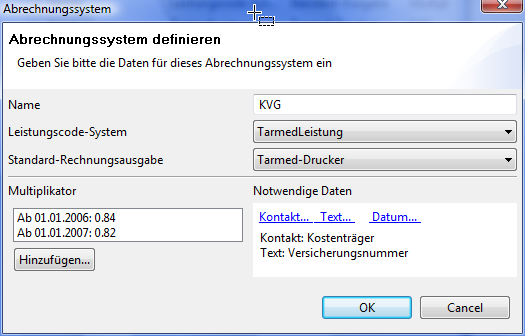
\includegraphics{abr2}\\
  \caption{KVG-Abrechnungssystem}\label{fig:abr2}
\end{figure}
Der Name ist wie gesagt frei wählbar. Für Leistungscode-System und Standard-Rechnungsausgabe können Sie aus den von den vorhandenen Abrechnungs-Plugins beigesteuerten Optionen wählen. Der Multiplikator ist die anzuwendende Tarifstufe (der 'Taxpunkt') für dieses System. Ein Multiplikator muss immer in Form einer Dezimalzahl angegeben werden und gilt immer ab einem bestimmten Datum so lange, bis ein anderer Multiplikator definiert wird. \textbf{Ein einmal eingegebener Multiplikator kann weder gelöscht noch geändert werden!}
\index{Taxpunkt}

Unter 'Notwendige Daten' geben Sie an, was für Angaben vorhanden sein müssen, damit ein Fall, der dieses Abrechnungssystem hat, als gültiog betrachtet wird. Solche Angaben können ein Kontakt sein, wie z.B. Kostenträger, oder ein Text, wie z.B. Versicherungs- oder Unfallnummer oder Vertragsnummer etc., oder es kann ein Datum sein, z.B. ein Unfalldatum.
Implizit immer notwendig ist der Kontakt 'Rechnungsempfänger', der deshalb hier nicht separat eingetragen werden darf.
Durch Rechtsklick kann man einen Eintrag in dieser Liste wieder löschen. Sie sehen das, was Sie hier eingegeben haben wieder unter den 'Fall-Details' als Fall-Erfordernisse (s. \ref{fall-erfordernisse}, S. \pageref{fall-erfordernisse}).

Unter 'Fallkonstanten' können je nach Abrechnungs-Plugin notwendige Daten eingetragen werden, die jedem auf diesem Abrechnungssystem basierenden Fall zugeordnet werden. Hier zum Beispiel das Gesetz, nach dem abgerechnet wird und die EAN des Intermediärs. Wenn der Hersteller Ihres Abrechnungsplugins hierzu keine Angaben gemacht hat, lassen Sie dieses Feld einfach leer.


\subsection{Mandanten und Rechnungssteller}
\index{Mandant}\index{Rechnungssteller}\index{Assistenzarzt}
Jeder Kontakt zwischen der Praxis und einem Patienten steht unter der Verantwortung eines \textit{Mandanten} und geht auf Rechnung eines \textit{Rechnungsstellers}. Im einfachsten und in der Schweiz üblichen Fall sind Mandant und Rechnungssteller identisch. Es ist aber auch möglich, dass ein Mandant im Fixlohn angestellt ist, auf eigen Verantwortung arbeitet, aber für einen anderen Rechnungssteller abrechnet (z.B. in einem HMO-Zentrum oder einer Polikinik). Dies ist nicht zu verwechseln mit einem Assistenten: Ein Assistent ist selber kein Mandant, sondern arbeitet auf Rechnung und unter der Verantwortung eines Mandanten.

\medskip

Einen Mandanten erstellt man, indem man ihn unter den \textit{Kontakten} anlegt und das Häkchen 'Mandant' ankreuzt. Danach kann man unter \textsc{Datei-Einstellungen-Mandanten} Benutzername und Passwort eingeben und festlegen, für welchen REchnungssteller dieser Mandant arbeitet.

Diese Zusammenhänge sind auch im Elexis-Handbuch beschrieben, genaueres bitte ich dort nachzulesen.

\medskip

Zurück zum Tarmed-System: Wenn das Plugin 'elexis-arzttarife-schweiz' installiert ist, finden Sie unter \textsc{Datei-Einstellungen-Abrechnungssysteme} auch die Positionen 'Labortarif', 'Physioterapie' und 'Tarmed-Rechnungen' (S. Abb. \ref{fig:abr1}). Wählen Sie zunächst den Punkt Labortarife (Abb. \ref{fig:abr3}):
\begin{figure}
  % Requires \usepackage{graphicx}
  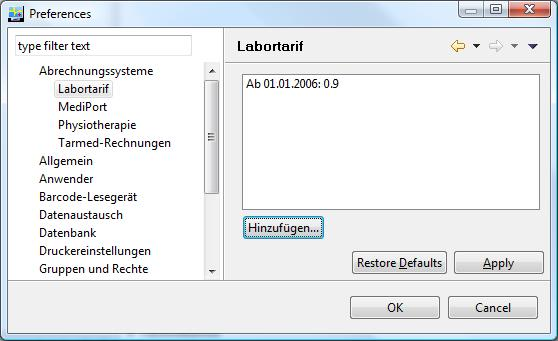
\includegraphics[width=0.95\textwidth]{abr3}\\
  \caption{Labor-Taxpunkt}\label{fig:abr3}
\end{figure}
Hier muss der Multiplikator gleich wie bei den Abrechnungssystemen eingegeben werden. Auch hier kann ein einmal eingetragener Wert nicht mehr geändert werden und er ist ab dem Stichdatum bis zur nächsten Änderung gültig.
\index{Taxpunkt}

\medskip

Für den Physiotherapie Tarif gehen Sie genau gleich vor wie beim Labortarif (Abb. \ref{fig:abr24}). Weitere Informationen finden Sie im Abschnitt \ref{physiotarif} auf Seite \pageref{physiotarif}
\begin{figure}
  % Requires \usepackage{graphicx}
  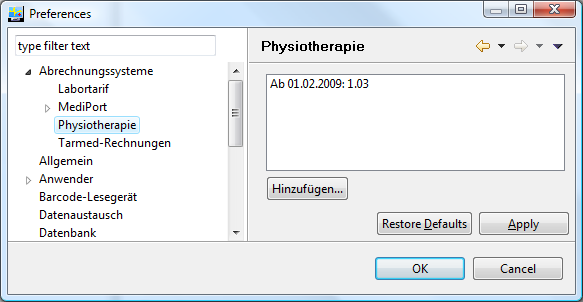
\includegraphics[width=0.95\textwidth]{abr24}\\
  \caption{Physio-Taxpunkt}\label{fig:abr24}
\end{figure}

\medskip

Gehen Sie dann zum Punkt 'Tarmed-Rechnungen'. Es erscheint ein Dialog wie in Abb.\ref{fig:abr4}.
\begin{figure}
    \center
  % Requires \usepackage{graphicx}
  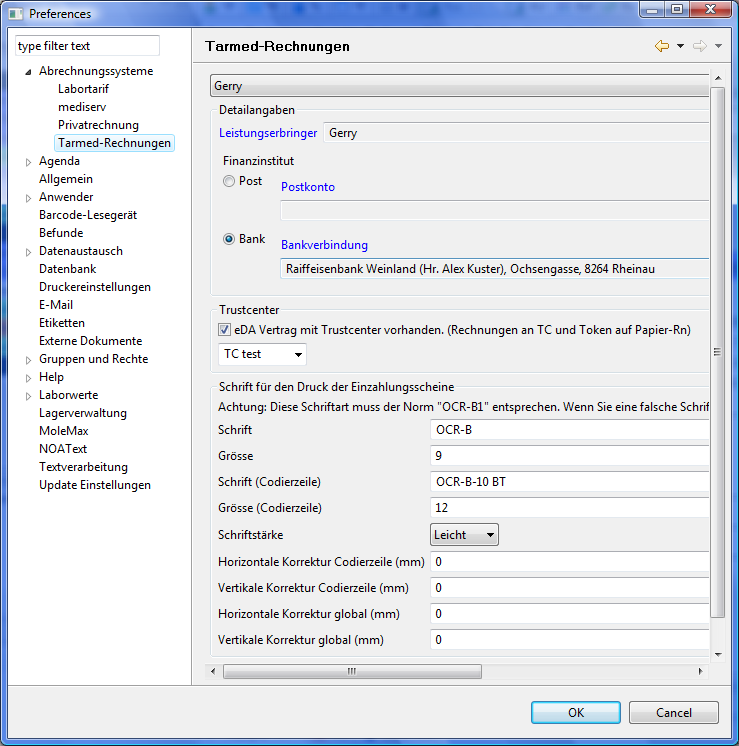
\includegraphics[width=0.95\textwidth]{abr4}\\
  \caption{Tarmedrechnungs-Einstellungen}\label{fig:abr4}
\end{figure}
\index{Leistungserbringer}\index{Mandant}\index{Rechnungssteller}
Hier müssen Sie für jeden Mandanten und Rechnungssteller \textit{separat} alle für die Abrechnung relevanten Daten eingeben. Wählen Sie also im Combobox-Feld ganz oben zunächst einen Mandanten aus. Dadurch erscheint im Feld hinter 'Leistungserbringer' der Name dieses Mandanten. Klicken Sie dann auf das blaue Wort 'Leistungserbringer'. Es öffnet sich eine Dialogbox wie in Abb \ref{fig:abr5}.
\begin{figure}
  % Requires \usepackage{graphicx}
  \center
  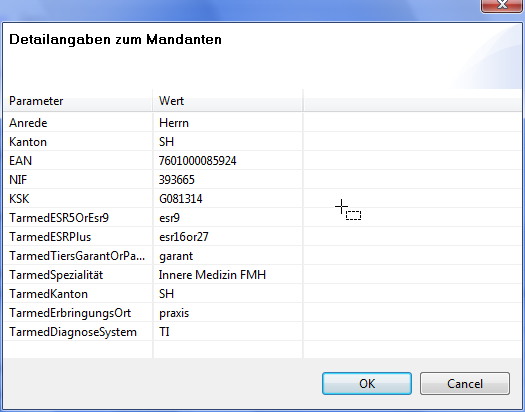
\includegraphics[width=0.75\textwidth]{abr5}\\
  \caption{Einstellung pro Mandant}\label{fig:abr5}
\end{figure}

Um eine Zeile zu ändern müssen Sie in dieser Zeile die \textbf{Eingabetaste} drücken, dann den neuen Wert eingeben, dann nochmal die \textbf{Eingabetaste} drücken und erst dann mit der Maus oder der Pfeiltaste ein anderes Feld aufsuchen.

Die Bedeutung der einzelnen Zeilen ist:
\index{EAN}\index{ZSR}\index{NIF}\index{ESR}
\begin{itemize}
\item Anrede: Sie haben es erraten ;-)
\item Kanton: Der Standort Ihrer Praxis. Wenn Sie in mehreren Kantonen praktizieren, müssen Sie einen eigenen Mandanten für jeden Kanton erstellen (z.B. Müller TI und Müller AG).
\item EAN: Ihre europäische Artikelnummer (Ja, wenn Sie ein in der Schweiz zugelassener Arzt sind, dann sind Sie auch ein europäischer Artikel, vergleichbar einer Milchtüte oder einem Badeschwamm). Falls Sie Ihre EAN nicht kennen, wenden Sie sich an die FMH.
\item NIF: Wenn Sie IV-Fälle behandeln, benötigen Sie eine Nummer der IV, die sich NIF nennt. Fragen Sie mich nicht, wieso die IV nicht die EAN verwenden kann.
\item KSK: Santésuisse hat Ihnen eine ZSR- oder KSK-Nummer gegeben, damit Sie über die Kassen abrechnen dürfen. Geben Sie diese Nummer ohne Punkte, Striche oder Leerzeichen ein. Und fragen Sie mich nicht, wieso Santésuisse nicht die EAN oder die NIF verwendet.
\item TarmedESR5OrEsr9: Das zu verwendende ESR-System. Fragen Sie  nicht, sondern schreiben Sie 'esr9'. Ausser, wenn Sie genau wissen, was Sie tun. Aber dann brauchen Sie eh nicht zu fragen.
\item TarmedEsrPlus: Dito. Schreiben Sie im Zweifelsfall einfach 'esr16or27'.
\item TarmedTiersGarantOrPayant: Schreiben Sie garant oder payant je nach Ihrem bevorzugten Abrechnungssystem. Hat aber zur Zeit nicht viel Konsequenz, was Sie da hinschreiben.
\item TarmedSpezialität: Der Titel, der Ihre 'Dignität' definiert. Fragen zum  Dignitätskonzept beantworten gerne und erschöpfend TarmedSuisse und die FMH.
\item TarmedKanton Nochmal der Praxisstandort.
\item TarmedErbringungsOrt praxis oder klinik (Wo Sie Ihre Leistungen erbringen)
\item TarmedDiagnoseSystem: Nach welcher Systematik Sie standardmässig Diagnosen auf den Rechnungen angeben. Schreiben Sie TI für Tessiner-Code, ausser wenn Sie einen guten und von TarmedSuisse abgesegneten Grund haben, etwas anderes zu schreiben.
\end{itemize}

Klicken Sie dann auf 'OK' um diesen Dialog wieder zu schliessen und wieder zu Abb.\ref{fig:abr4} zurückzukommen.


\subsection{Post- oder Bankkonto}
\index{Bankkonto}\index{Postkonto}\index{VESR}\index{BESR}\index{ESR}
Jetzt müssen Sie das Konto angeben, auf das Sie die Zahlungen für Ihre Rechnungen erwarten. Sie benötigen ein VESR oder BESR Konto, zusammenfassend auch ESR-Konto genannt. Ein VESR-Konto ist ein ESR-Konto bei der Post, ein BESR-Konto ist eines bei einer Bank. Ein ESR-Konto ist eines, das mit diesen orangen (früher blauen) Einzahlungsscheinen befüllt wird, auf denen eine Referenznummer steht und deren Mitteilungskästchen mit einem vorgedruckten 'Keine Mitteilungen anbringen' beschriftet ist.

Das schöne an ESR-Konti ist, dass Dateien mit Zahlungseingängen automatisch eingelesen und verarbeitet werden können, so dass Sie die Zahlungen nicht manuell verbuchen müssen, sondern diese Aufgabe an den Computer delegieren können.

\medskip

 \textbf{Dringende Empfehlung} Falls Sie schon ein ESR-Konto haben, das Sie mit einem anderen Programm benutzen, eröffnen Sie ein neues für die Benutzung mit Elexis, weil sonst die ESR-Zeilen nicht bzw. falsch interpretiert werden und beide Programme bei jedem Einlesen Fehlermeldungen ausspucken werden!

\medskip

Eröffnen Sie also je nach Geschmack bei der Post oder Ihrer Lieblingsbank ein ESR-Konto. Klicken Sie je nachdem auf das blaue Wort 'Postkonto' oder 'Bankverbindung'\footnote{Im Fall von 'Bankverbindung' muss Ihre Bank zuvor als Kontakt erfasst worden sein}.

\begin{figure}[htbp]
     \begin{minipage}{0.5\textwidth}
      \centering
       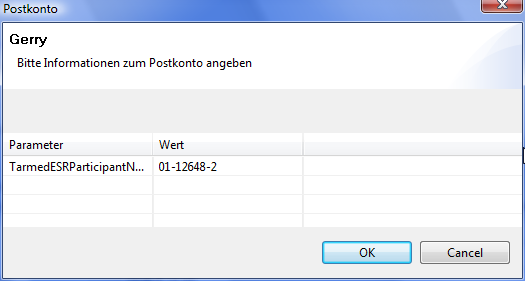
\includegraphics[width=0.95\textwidth]{abr6}
       \caption{VESR (Post)}
       	\label{fig:abr6}
     \end{minipage}\hfill
     \begin{minipage}{0.5\textwidth}
      \centering
       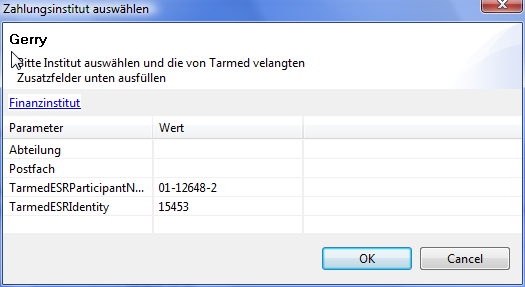
\includegraphics[width=0.95\textwidth]{abr7}
       \caption{BESR (Bank)}
       \label{fig:abr7}
     \end{minipage}
   \end{figure}

Je nach Auswahl erscheint eine Dialogbox wie Abb. \ref{fig:abr6} oder Abb. \ref{fig:abr7}. Beim Postkonto müssen Sie nur die VESR-Teilnehmernummer eintragen, die Sie von der Post erhalten haben. Beim Bankkonto benötigen Sie zunächst die Bank: Klicken Sie auf das blaue 'Finanzinstitut' und wählen Sie den hoffentlich zuvor angelegten Kontakt, der Ihre Bank beschreibt. Geben Sie dann neben TarmedESRParticipantNumber die VESR-Teilnehmernummer \textit{der Bank} ein. Neben TarmedESRIdentity müssen Sie die BESR-Identitätsnummer eingeben, die Sie von der Bank bekommen haben. Klicken Sie dann auf OK, um wieder zu Abb. \ref{fig:abr4} zurückzukommen.

\subsection{TrustCenter}
\index{TrustCenter}
Da gibt es nicht viel zu sagen. Falls Sie einen TC-Vertrag haben, setzen Sie hier ein Häkchen und wählen Ihr TrustCenter aus. (Wenn Sie das tun, dann wird auf dem Rückforderungsbeleg von TG-Rechnungen ein passendes Token gedruckt, das beinahe wie eine ESR-Zeile aussieht, aber keine ist).

\subsection{Einzahlungsschein}
\index{ESR-Papier}
Elexis benötigt a4-Papier mit \textit{unten} integriertem ESR-Einzahlungsschein. Also das unterste Drittel der A4-Seite ist der orange Einzahlungsschein des Typs BESR oder VESR (bei ersterem steht eine Zeile 'zugunsten von' im Empfänger-Feld).

\index{OCR-Schriftart}
Zunächst benötigen Sie eine Schriftart des Typs OCR-B. diese Schriftart muss auf dem Computer installiert sein, von dem aus die Rechnungen gedruckt werden sollen \footnote{Tatsächlich empfehlen wir ausdrücklich, Rechnungen immer vom selben PC auf denselben Drucker auszugeben. Erst wenn das reibungslos funktioniert, können Experimente mit unterschiedlichen PC's gemacht werden, wenn es unbedingt sein muss.}. Nein, diese Schriftart ist nicht Bestandteil von Elexis, da sie lizenzpflichtig ist. Möglicherweise haben Sie aber von einem anderen ESR-fähigen Programm eine solche Schriftart irgendwo installiert und können diese verwenden. Ansonsten können Sie sich auch an die Post oder Ihre Bank wenden um zu erfahren, wo Sie diese Schriftart kaufen können.


Weil unterschiedliche Drucker das Papier nicht hunterprozentig identisch positionieren, und weil die Post ein wenig kritisch bezüglich der
Position der ESR-Zeile ist, kann man ausserdem den Ausdruck hier entsprechend konfigurieren. Sie benötigen ev eine ESR-Schablone, auf der Sie die korrekte Grösse und Positionierung der Codierzeile ablesen können.

Nun zu den Einstellungen:
\begin{itemize}
\item Unter 'Schrift' geben Sie diejenige Schriftart ein, die der Einzahlungsschein ausserhalb der ESR-Zeile haben soll. Nehmen Sie hier irgendetwas nach Ihrem Geschmack (es muss natürlich eine auf dem PC installierte Schriftart sein).
\item Unter 'Grösse' geben Sie die gewünschte Schriftgrösse in Punkt ein.
\item Unter 'Schrift (Codierzeile)' müssen Sie die OCR-B Schriftart angeben.
\item Mit 'Grösse (Codierzeile)' und der 'Schriftstärke' müssen Sie etwas experimentieren, bis Sie die korrekte OCR-lesbare Zeile haben
\item Horizontale Korrektur der Codierzeile: Mit positiven Werten schieben Sie die Codierzeile nach rechts, mit negativen nach links.
\item Vertikale Korrektur der Codierzeile: Mit positiven Werten schieben Sie die Zeile nach unten, mit negativen nach oben.
\item Horizontale Korrektur global: Wenn besipielsweise die Zahlen nicht schön in die Felder kommen, können Sie hier den Einzahlungsschein als ganzes verschieben. (Sie müssen danach allerdings vermutlich die Codierzeile wieder neu positionieren).
\item vertikale Korrektur global: Den ganzen Einzahlungsschein-Inhalt nach oben oder unten verschieben.
\end{itemize}

Dann können Sie diese Dialogbox schliessen.

\subsection{Druckvorlagen}
\index{Rechnungsvorlagen}
Wie (fast) alles, was in Elexis ausgedruckt wird, basieren auch Rechnungen auf Druckvorlagen. Bei Tarmed heissen diese System-Vorlagen:

\medskip

\begin{tabular}{|l|l|}
\hline
Tarmedrechung\_EZ & Tarmedrechnung mit ESR\\
Tarmedrechnung\_M1 & Erste Mahnung mit ESR\\
Tarmedrechnung\_M2 & Zweite Mahnung mit ESR\\
Tarmedrechnung\_M3 & Dritte Mahnung mit ESR\\
\hline
Tarmedrechnung\_S1 & Rückforderungsbeleg/TP-Rechnung erste Seite\\
Tarmedrechnung\_S2 & Rückforderungsbeleg/TP-Rechnung Folgeseite\\
\hline

\end{tabular}

\medskip

Diese Vorlagen sollten mit der Installation bereits vorhanden sein. Sie können die oberen 4 anpassen, aber es dürfen nur die oberen zwei Drittel des Blattes verwendet werden (das unterste Drittel wird der Einzahlungsschein). Achtung: Wenn Sie mehrere Mandanten haben und mandantenspezifische Texte verwenden, dann müssen Sie jede Vorlage mehrmals, einmal für jeden Mandanten, speichern. (Standardmässig sind die Rechnungsvorlagen für 'alle' gespeichert)

Die Seiten S1 und S2 sollten wenn überhaupt nur sehr vorsichtig geändert werden, da das Layout nicht geändert werden darf. Andernfalls sind es keine gültigen Tarmed-Rechnungen mehr.

Wie immer müssen Sie, wenn Sie eine Systemvorlage geändert haben, diese anschliessend explizit mit 'als Vorlage speichern... Systemvorlage' zurückspeichern, sonst gehen die Änderungen verloren.

\subsubsection{Druckvorlagen auf Drucker konfigurieren}
\label{druckkonfiguration}
\index{Drucken!Vorlagen}
\index{Drucken!Korrektur}
\index{Drucken!Schacht}
Sie müssen Elexis mitteilen, auf welchem Drucker und in welchem Schacht die Seiten mit ESR-Papier und die weissen Seiten ausgedruckt werden sollen. Beim NOAText-Plugin (Das ist das Textsystem, welches standardmässig unter Windows installiert ist), erfolgt diese Einstellung \textit{nicht} wie vielleicht erwartet unter \textsc{Datei-Einstellungen-Drucker}, sondern bei der Druckvorlage. Die Optionen unter \textsc{Datei-Einstellungen-Drucker} betreffend A4-Papier und ESR-Papier müssen in diesem Fall vielmehr sogar leer gelassen werden, damit die Druckkonfiguration gelingt!

\medskip

Um das Druckziel einzustellen, gehen Sie so vor: Laden Sie die betreffende Systemvorlage, z.B. 'Tarmedrechnung\_EZ' mit dem Menüpunkt \textsc{Systemvorlage laden} im lokalen Menu der Briefe-View. Wählen Sie dann im OpenOffice-Menu dieses Dokuments \textsc{Datei-Drucken...}. Geben Sie im Druckdialog unter 'Eigenschaften' den richtigen Drucker und Schacht ein.  Drucken Sie sie dann aus und schauen Sie, ob sie wirklich aus dem erwarteten Drucker und Schacht gedruckt wird. \textbf{Speichern} Sie dann die Vorlage wieder als Systemvorlage, und zwar unter demselben Namen, den sie vorher hatte. Wiederholen Sie diese Schritte für alle oben genannten Tarmedrechnungs-Vorlagen. (Dabei müssen \_S1 und \_S2 natürlich auf dem Schacht für weisses Papier ausgegeben werden, die anderen aus dem Schacht für ESR-Papier).

\section{Schritt für Schritt: Verrechnen, Rechnungen erstellen und ausgeben}
\label{rechnungenerstellen}
\subsection{Fälle, Rechnungsempfänger und Kostenträger}
\index{Fall}
Ein 'Fall' ist die Zuordnung eines Patienten zu einem Kostenträger und einer Identifikation des Kostenträgers für den Fall. Beispiel: Patient, Krankenkasse und Versicherungsnummer für KVG-Behandlungen oder Patient, Versicherung und Unfallnummer für UVG-Behandlungen, oder Patient, IV-Stelle und AHV-Nummer für IV-Behandlungen.

\medskip

Damit bleibt ein Fall auch immer so lange gültig, wie die Behandlungen demselben Versicherungsereignis zugeordnet bleiben. Ein KVG-Fall also bis der Patient die Kasse wechselt, ein UVG-Fall bis der Unfall abgeschlossen ist. Das Erstellen von Rechnungen hängt zunächst nicht damit zusammen -- Ein und derselbe Fall kann keine, eine oder mehrere Rechnungen haben. Es werden immer automatisch alle noch nicht verrechneten Konsultationen auf die nächste Rechnung genommen. (Ausser, wenn man es manuell anders macht).

\medskip

\textbf{Wichtig:} Ein einmal erstellter Fall ist wie ein Krankenkassenkärtli oder ein
\index{Fall!ändern} Unfallschein zu betrachten. Das heisst, er darf nicht mehr geändert werden.\footnote{Selbstverständlich ist es gestattet, fehlende Angaben später nachzutragen, oder Tippfehler zu korrigieren, wenn etwa die Versicherungsnummer sich nicht geändert hat, aber falsch eingegeben worden ist} Wenn sich etwas an der Versicherung ändert, muss ein neuer Fall erstellt werden.

\subsubsection{Fall-Eigenschaften}
\label{fall-erfordernisse}
\begin{figure}
  % Requires \usepackage{graphicx}
  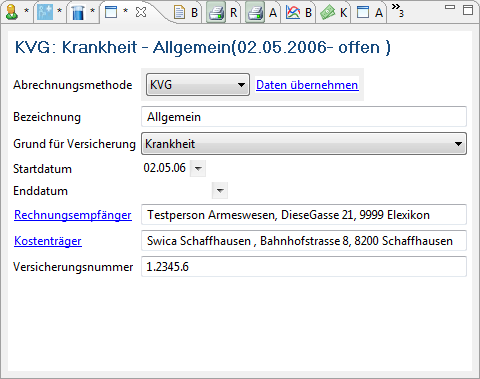
\includegraphics[width=0.7\textwidth]{abr8}\\
  \caption{Fall-Detail}\label{fig:abr8}
\end{figure}
\index{Fall!Eigenschaften}
Ein Fall ist immer einem Abrechnungssystem zugeordnet. Beim Erstellen eines neuen Falls muss im obersten Feld die 'Abrechnungsmethode' angegeben werden (s. Abb.\ref{fig:abr8}).
Darunter geben Sie eine Bezeichnung ein. Diese ist nur zur internen Markierung des Falles gedacht, damit Sie wissen, welcher Fall gemeint ist. Sie können hier irgendetwas schreiben, z.B. 'Beinbruch'.
Darunter das Feld 'Grund für die Versicherung' ist ein Tarmed-Erfordernis und wird auf der Rechnung erscheinen.
\textit{Startdatum} ist bei Unfällen idR das Unfalldatum, bei KVG-Behandlungen die erste Konsultation.
\index{Fall!Abschliessen}
\textit{Enddatum} ist nur anzugeben, wenn der Fall abgeschlossen wird, also z.B. der Unfall abgeschlossen ist oder die Kasse gewechselt wird. Sobald ein Enddatum angegeben ist, ist der Fall als 'geschlossen' markiert und kann keine weiteren Konsultationen mehr aufnehmen.
Die nächsten Zeilen betreffen die für die Rechnungsstellung erforderlichen Daten. Diese hängen davon ab, was beim Erstellen des Abrechnungssystems dieses Falles definiert wurde.
Immer erforderlich ist der \textit{Rechnungsempfänger} - Wenn es keinen Rechnungsempfänger gibt, kann Elexis keine Rechnung erstellen.
Alle anderen Angaben hängen wie gesagt vom Abrechnungssystem ab.

Elexis betrachtet einen Fall als ungültig, wenn nicht alle Erfordernisse angegeben sind. Der Fall ist dann mit einem roten Punkt markiert. Wenn alle Erfordernisse eingetragen sind, wird der Punkt grün.

\subsubsection{Tiers Garant und Tiers Payant}
\index{Tiers Garant}\index{Tiers Payant} \index{Tiers Soldant} \index{TG}\index{TP}\index{Rechnungsempfänger}\index{Kostenträger}
Tiers Payant bedeutet: Rechnungsempfänger und Kostenträger sind identisch. Tiers Garant bedeutet: Der Rechnungsempfänger ist nicht identisch mit dem Kostenträger. Es kann der Patient selbst sein, oder dessen Vormund, oder das Sozialamt. Tiers Soldant ist wiederum eine Variante von Tiers Payant, bei der der Kostenträger den nicht dem Selbstbehalt unterworfenen Anteil der Rechnung direkt an den Leistungserbringer zahlt.

Sie legen also beim Erstellen eines Falles fest, ob eine TP-Rechnung oder eine TG-Rechnung mit Rückforderungsbeleg erstellt wird: Wenn Sie für Kostenträger und Rechnungsempfänger denselben Kontakt auswählen, wird es TP, sonst TG.

\subsection{Rechnungen erstellen}
Es gibt zwei prinzipiell gleichwertige Möglichkeiten, Rechnungen zu erstellen: Sofortrechnung und (halb-)automatischer Rechnungslauf.

\subsubsection{Sofortrechnung}
\index{Sofortrechnung}
Klicken Sie mit der rechten Maustaste in der 'Fälle'-View auf den Fall und wählen Sie 'Rechnung erstellen'. Es wird direkt eine Rechnung über alle noch offenen Konsultationen des aktuellen Mandanten des gewählten Falles erstellt.

\subsubsection{(halb-)automatischer Rechnungslauf}
\index{Rechnungslauf}
Gehen Sie in die Rechnungen-Perspektive und öffnen Sie die View 'Konsultationen zum Verrechnen'. Hier findet sich in der linken Hälfte eine Liste aller noch unverrechneter Konsultationen des aktuellen Mandanten, gruppiert nach Patienten und Fällen. In der rechten Hälfte findet sich eine Liste derjenigen Konsultationen, die zum Rechnungserstellen vorgemerkt sind. Es gibt nun verschiedene Möglichkeiten, Konsultationen zwischen der linken und der rechten Liste zu verschieben:
\begin{itemize}
\item Alle Konsultationen aller Fälle eines Patienten: Ziehen Sie mit der Maus einen Patienteneintrag von der linken in die rechte Hälfte. Wenn Sie mehrere Patienten gleichzeitig auswählen wollen, können Sie wie in Windows gewohnt mit Druck auf die Shift- oder Ctrl-Taste und Mausklick mehrere auswählen und dann gemeinsam nach rechts ziehen. (Um \textit{alle} auszuwählen klicken Sie zunächst auf den ersten, dann mit 'Shift' auf den letzten Eintrag der Liste).
\item Alle Konsultationen eines Falles eines Patienten: Klicken Sie auf das (+)-Zeichen neben dem Patientennamen. Sie sehen alle Fälle, die noch unverrechnete Konsultationen enthalten. Ziehen Sie den gewünschten Fall in die rechte Hälfte.
\item Einzelne Konsultationen: Klicken Sie auf das (+)-Zeichen neben dem Fall. Sie sehen alle noch unverrechneten Konsultationen dieses Falles. Ziehen Sie eine oder mehrere ins rechte Feld.
\item Alle Konsultationen, die innerhalb eines bestimmten Zeitraums liegen: Öffnen Sie das View-Menu und wählen Sie 'Nach Datum auswählen'. Geben Sie in der dann öffnenden Dialogbox (Abb.\ref{fig:abr10}) das gewünschte Anfangs- und Enddatum ein.
\begin{figure}
  % Requires \usepackage{graphicx}
  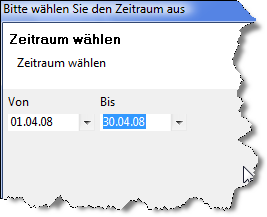
\includegraphics{abr10}\\
  \caption{Konsultationen nach Datum auswählen}\label{fig:abr10}
\end{figure}

\item Automatische Auswahl anhand verschiedener Kriterien: Klicken Sie das 'Zauberstab-Icon' und wählen Sie aus der Dialogbox wie Abb.\ref{fig:abr9} die gewünschten Kriterien aus:
\begin{figure}
  % Requires \usepackage{graphicx}
  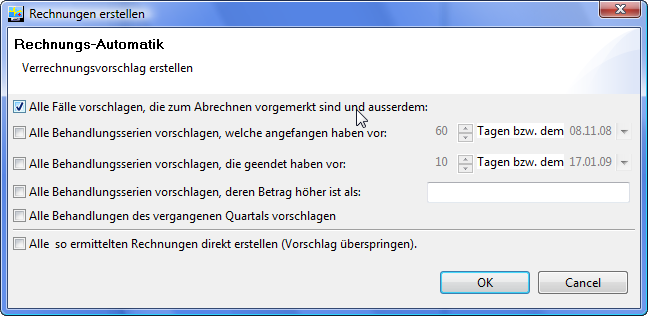
\includegraphics[width=1.0\textwidth]{abr9}\\
  \caption{Konsultationen automatisch auswählen}\label{fig:abr9}
\end{figure}
\begin{itemize}
    \item Alle Konsultationen, deren Fall manuell zum Abrechnen vorgemerkt wurde (Im Fall-Detail)
    \item Alle Konsultationen einer Serie, deren erste vor einem bestimmten Datum war
    \item Alle Konsultationen einer Serie, deren letzte vor einem bestimmten Datum war
    \item Alle Konsultationen des vergangenen Kalenderquartals
    \item Alle Konsultationen, deren summierter Betrag eine bestimmte Höhe überschreitet.
    \end{itemize}
\end{itemize}

Je nach Gewohnheiten Ihrer Praxis werden Sie vermutlich nicht alle diese Methoden anwenden. In jedem Fall haben Sie anschliessend eine Anzahl Patienteneinträge in der rechten Hälfte des Fensters. Bis zu diesem Zeitpunkt ist noch nichts 'irreversibles' passiert. Sie können einzelne Einträge wieder entfernen, indem sie sie mit der rechten Maustaste anklicken und 'aus Auswahl entfernen' wählen. Sie können auch die ganze Auswahl wieder leeren, indem Sie auf das rote X - Symbol klicken. Oder Sie können die Liste der Rechnungen in der Auswahl ausdrucken, indem Sie auf das Druckersymbol klicken.

\medskip

\index{Rechnung!erstellen}
Wenn Sie sicher sind, dass alles stimmt, können Sie nun aus der Auswahl Rechnungen erstellen lassen. \textbf{Achtung:} Dieser Schritt ist nicht mehr reversibel. Einmal erstellte Rechnungen können nicht mehr 'ungeschehen' gemacht werden. Klicken Sie also auf den Button 'Rechnungen erstellen'.
Wenn Sie unter \textsc{Datei-Einstellungen-Abrechnungssysteme} den Punkt 'Strenge Gültigkeitsprüfung beim Rechnungserstellen  angekreuzt hatten, erfolgt vor dem Rechnungserstellen noch eine Konformitätsprüfung (welche  vom gewählten Abrechnungssystem abhängt). Bei Rechnungen nach Tarmed wird z.B. geprüft, ob die EAN des Kostenträgers angegeben ist und ob eine Rechnungsdiagnose vorhanden ist. Bei Fehlern wird die Rechnung nicht erstellt und die Konsultationen bleiben offen. (Es erscheint eine entsprechende Fehlermeldung für jede Rechnung, die nicht erstellt werden kann).
\index{Rechnung!Gültigkeitsprüfung}
Wenn die 'Strenge Gültigkeitsprüfung' nicht angekreuzt ist, genügt es, wenn ein Rechnungsempfänger vorhanden ist, um die Rechnung zu erstellen.

\medskip

\textbf{Wichtig:} Elexis lässt Ihnen zwar die Wahl, wie 'stur' Sie beim Prüfen der Rechnungsvoraussetzungen sein wollen, aber dies hat natürlich keinerlei Einfluss darauf, wie 'stur' die Gegenseite ist. Eine Rechnung, die nicht Tarmed-Konform ist, kann vom TrustCenter oder der Kasse zurückgewiesen werden. Dies ist dann kein Fehler von Elexis, sondern von den fehlenden Daten. Wenn Sie die 'strenge Prüfung' eingeschaltet lassen, wird Elexis nur Tarmed-Konforme Rechnungen erstellen\footnote{Fehler wie immer vorbehalten}, aber Sie dafür mit Fehlermeldungen 'nerven', wenn die Daten nicht konform sind.

\subsection{Rechnungen anzeigen, kontrollieren und ausgeben}
\index{Rechnung!kontrollieren}
Wenn Sie eine Rechnung erstellt haben, durchläuft sie einen Zyklus von verschiedenen Statusänderungen, bis sie schliesslich einen Endpunkt erreicht hat. Zunächst hat sie den Status 'Offen'\footnote{Eine Ausnahme sind Rechnungen, deren Totalbetrag 0.00 ist: Solche Rechnungen werden automatisch unmittelbar nach dem Erstellen auf den Status 'bezahlt' gesetzt.}. Das bedeutet, sie wurde erstellt, aber noch nirgendwohin übermittelt oder ausgegeben. Sie finden alle Rechnungen in der View 'Rechnungen' (S. Abb.\ref{fig:abr11}), welche standardmässig in der Abrechnungs-Perspektive vorhanden ist (Aber natürlich auch in jede andere Perspektive eingebaut werden kann).
\begin{figure}
  % Requires \usepackage{graphicx}
  \center
  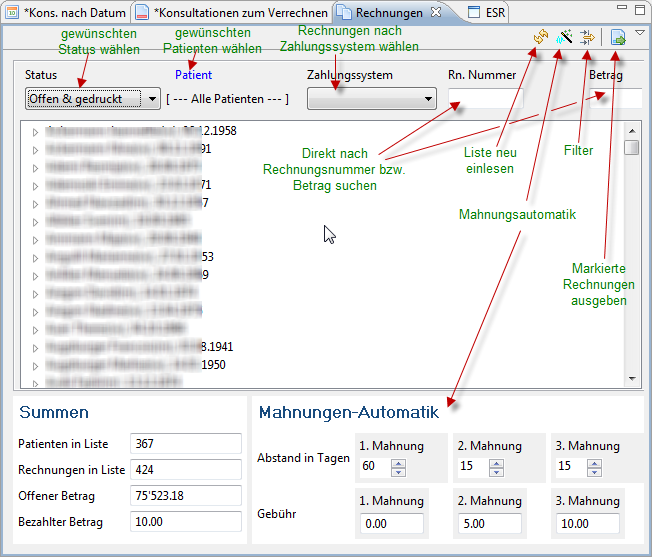
\includegraphics[width=0.9\textwidth]{abr11}\\
  \caption{Rechnungen-View}\label{fig:abr11}
\end{figure}
\begin{figure}
  % Requires \usepackage{graphicx}
  \center
  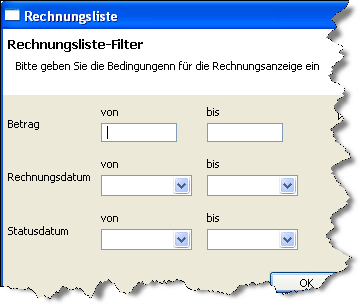
\includegraphics[width=5.5cm]{abr12}\\
  \caption{Rechnungsliste-Filter}\label{fig:abr12}
\end{figure}

Wie Sie sehen, können Sie die Liste der Rechnungen nach bestimmten Kriterien Filtern. Nach jeder Änderung des Filters kann die Liste mit dem 'Neu einlesen'-Button wieder unter Anwendung der geänderten Filterbedingungen neu eingelesen werden.

\begin{itemize}

\item Mit der Combobox ganz links kann die Liste nach Status gefiltert werden. Alle neu erstellten Rechnungen finden Sie beispielsweise unter dem Status 'Offen', alle bezahlten Rechnungen unter dem Status 'bezahlt' usw.

\item Mit dem nächsten Feld 'Patient' können nur Rechnungen eines bestimmten Patienten angezeigt werden. Nach Klick auf das blaue Wort 'Patient' öffnet sich ein Dialog, in dem Sie den gewünschten Patienten auswählen können. Wenn Sie in diesem Dialog 'Abbrechen' bzw. 'Cancel' klicken, wird der Filter wieder auf 'Alle Patienten' gesetzt, ansonsten auf den ausgewählten Patienten.

\item Mit der Combobox 'Zahlungssystem' können nur Rechnungen eines bestimmten Zahlungssystems angezeigt werden. Wenn Sie beispielsweise das Zahlungssystem auf 'UVG' und den Status auf 'Offen' setzen und die Liste neu einlesen, können Sie einen Rechnungslauf mit allen offenen UVG-Rechnungen machen.

\item Im Feld 'RnNummer' könne Sie direkt eine Rchnungsnummer eingeben und die Eingabetaste drücken, um die genannte Rechnung aufzurufen.

\item mit dem 'Filtern'-Button können Sie eine weitere Dialogbox aufrufen (Abb.\ref{fig:abr12}), um weitere  Bedingungen für den Filter einzugeben:
    \begin{itemize}
    \item Betrag von-bis: Geben Sie jeweils einen Betrag in der Form x.xx ein. Es werden diejenigen Rechnungen ausgewählt, deren Totalbetrag zwischen diesen beiden liegt.
    \item Rechnungsdatum von-bis: Geben Sie jeweils ein Datum ein (Durch Klick auf das Dreieck öffnet sich ein Kalender). Es werden diejenigen Rechnungen angezeigt, die zwischen diesen Daten erstellt wurden. Sie können auch das erste Feld leer lassen, dann werden alle ausgewählt, die irgendwann vor dem im zweiten Feld genannten Datum erstellt wurden, oder sie können das zweite Feld leer lassem, dann werden alle irgendwann nach dem Datum im ersten Feld ausgegeben.
    \item Statusdatum von-bis: Gleich wie Rechnungsdatum, aber es wird das Datum der letzten Statusänderung als Kriterium genommen.
    \end{itemize}

\end{itemize}


Je nach Filterung werden in der Liste nun alle Patienten angezeigt, welche Rechnungen haben, die den genannten Kriterien entsprechen. Wenn Sie einen Patienteneintrag mit der rechten Maustaste anklicken, können Sie die View Patient-Details aufrufen. Durch Klick auf das (+)-Symbol können Sie anzeigen lassen, welche Fälle davon betroffen sind. Durch KLick mit der rechten Maustaste auf einen Fall können Sie sich die Falldetails anzeigen lassen, und durch Klick auf das (+) Symbol vor den Fällen können die einzelnen Rechnungen angezeigt werden. Durch Rechtsklick auf eine Rechnung kommen Sie zum Rechnungs-Menü, auf das wir später noch zurückkommen werden.

\medskip

\index{Rechnung!kontrollieren}
Wenn eine Rechnung angeklickt wird, können die Details der Rechnung angezeigt werden, wenn die Rechnungsdetail-View offen ist (Abb.\ref{fig:abr13}).
\begin{figure}
  % Requires \usepackage{graphicx}
  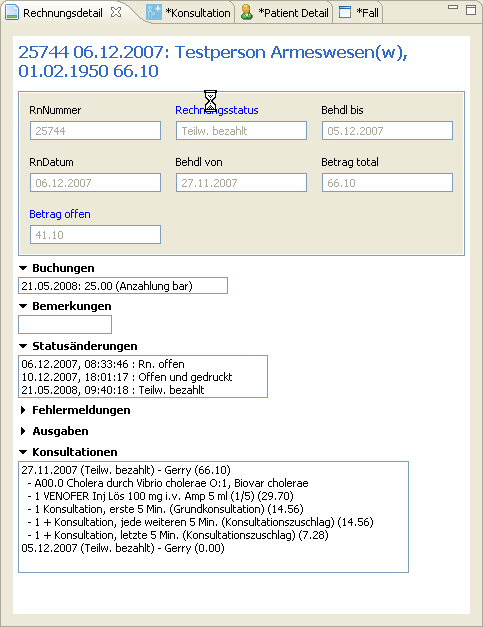
\includegraphics[width=0.9\textwidth]{abr13}\\
  \caption{Rechnungsdetail}\label{fig:abr13}
\end{figure}

Die Felder im oberen Abschnitt sollten selbsterklärend sein. Unten finden sich mehrere aufklappbare Felder.
\begin{itemize}
\item Buchungen: Alle Buchungen für diese Rechnung, ggf. mit einem Buchungstext
\item Bemerkungen: Hier können Sie beliebige Bemerkungen eingeben, z.B. Gründe für manuelle Statusänderungen oder Zahlungsaufschub etc. Diese Bemerkungen erscheinen nicht auf der Rechnung, sondern dienen nur der persönlichen Information in der Rechnungsdetail-View.
    \index{Rechnung!Bemerkungen}
\item Statusänderungen: Datum und Zeit jeder Änderung des Rechnungsstatus, sowie Bezeichnung des neuen Status.
\item Fehlermeldungen: Falls es bei der Rechnungsausgabe zu Fehlern gekommen ist, genauere Bezeichnung des Fehlers.
\item Ausgaben: Alle bisher erfolgten Ausgaben mit Datum, Zeit und Ausgabeziel dieser Rechnung.
\item Konsultationen: Sämtliche Verrechnungspositionen und Diagnosen der mit dieser Rechnung erfassten Konsultationen.
\end{itemize}

\subsubsection{Rechnungen zur Ausgabe auswählen}
Wählen Sie nun in der Rechnungsliste-View alle Patienten, Fälle oder Einzelrechnungen aus, die Sie ausgeben wollen. Wie gewohnt können Sie entweder einzelne Einträge mit der linken Maustaste auswählen, oder mit gleichzeitiger CTRL-Taste mehrere oder mit gleichzeitiger Shift-Taste ganze Reihen selektieren.

\medskip

Klicken Sie dann auf den Button 'Rechnungen ausgeben'. Es öffnet sich der Rechnungsausgabe-Dialog (Abb.\ref{fig:abr14}).
\begin{figure}
  % Requires \usepackage{graphicx}
  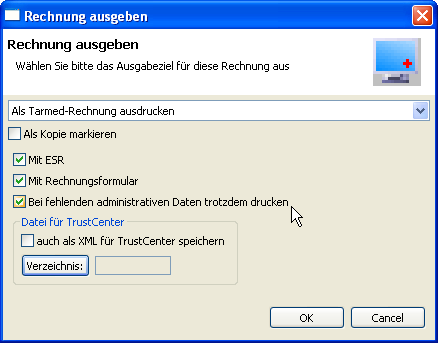
\includegraphics{abr14}\\
  \caption{Rechnungs-Ausgabe}\label{fig:abr14}
\end{figure}
Hier müssen Sie zunächst das passende Rechnungsausgabeziel auswählen, wobei die beim letzten Mal getroffene Wahl als Vorgabe erscheint.

\subsubsection{Ausgabeziele}
\index{Rechnung!ausgeben}\index{Rechnung!drucken}
Eine Rechnung kann auf verschiedene Ziele ausgegeben werden. Ein Rechnungsziel kann etwa der Drucker sein, oder auch ein Rechnungsintermediär, oder ein TrustCenter oder auch einfach eine Datei, die einem anderen Programm zur Weiterverarbeitung übergeben werden kann. Das Standard-Ausgabeziel wird mit der Wahl der Abrechnungsmethode eines Falles vorgegeben, man kann aber auch auf andere Ziele ausgeben. Man kann eine Rechnung oder eine Rechnungsserie auch erst auf eines und danach noch auf ein anderes Ziel ausgeben. Welche Ausgabeziele vorhanden sind, hängt von den installierten  Abrechnungsplugins ab. Wenn Sie elexis-arzttarife-schweiz installiert haben, sind die Ausgabeziele 'Als Tarmed-Rechnung ausdrucken' und 'Tarmed XML-4.0 Datei für TrustCenter' vorhanden, und ich werde im Folgenden diese beiden kurz beschreiben.

\subsubsection{Ausgabe auf Drucker}
Dies wird nur dann gelingen, wenn die Druckformatforlagen korrekt installiert und auf den Drucker eingestellt worden sind (Vgl. \ref{druckkonfiguration} auf S. \pageref{druckkonfiguration}). Sie können wählen, ob Sie die Seite mit dem Einzahlungsschein ('Mit ESR') oder den Rückforderungsbeleg resp. das TP-Rechnungsformular ('Mit Rechnungsformular') oder beides ausdrucken wollen. Falls Sie bei UVG-Rechnungen keinen Einzahlungsschein benötigen, können Sie z.B. alle UVG-Rechnungen auswählen und mit diesen einen Rechnungslauf mit nur dem Rechnungsformular machen.
Ausserdem können Sie noch angeben, ob die Rechnung 'als Kopie' markiert werden soll. Das empfiehlt sich dann, wenn ein Patient einen Zweitausdruck verlangt weil der erste verlorengegangen ist: Es werden dann Rückfragen vermieden, falls das Formular doch zweimal bei der Kasse eingereicht wird.

\medskip

Last but not least können Sie im untersten Abschnitt der Dialogbox noch festlegen, dass die Rechnung zusätzlich zum Ausdruck auch als XML-Datei fürs TrustCenter gespeichert werden soll.
Da TrustX aus irgendwelchen Gründen einen proprietären Layer um die verwendeten Übermittlungsdienste gepackt hat, kann die Übermittlung nur mit dem von TrustX bereitgestellten Programm erfolgen\footnote{Im Prinzip kann mann das TrustX-Modul auch einbinden, wie das vom elexis-trustx Plugin gemacht wird. Ich rate davon inzwischen allerdings ab: Da das TrustX-Modul unter Vista Administratorrechte verlangt, ist es eine potentielle Sicherheitslücke. Und wenn es Teil von Elexis wäre, müssten Sie Elexis selbst ebenfalls mit Administratorrechten starten, was ich vom Sicherheitsstandpunkt her inakzeptabel fände.}. Sie können es hier herunterladen (für windows):
\begin {verbatim}
 http://www.trustx.ch/trustx-praxis/documents/trustx-2_1_14-de.msi
\end{verbatim}
Wenn Sie dieses Programm installieren und gemäss Anleitung konfigurieren (Unter Vista müssen Sie es so konfigurieren, dass es im Kompatibilitätsmodus läuft und Administratorrechte bekommt), dann legt es unter anderem auch ein Verzeichnis für Rechnungen an (z.B. c:$\backslash$programme$\backslash$arpage$\backslash$trustx$\backslash$rechnungen)
Klicken Sie unter Elexis im Ausgabe-Dialog  (Abb.\ref{fig:abr14}) auf den 'Verzeichnis'-Knopf und suchen Sie dieses Verzeichnis auf. Dann können Sie ein Häkchen bei 'auch als XML-Datei für TrustCenter speichern' setzen. Elexis merkt sich die gewählte Einstellung und das Verzeichnis fürs nächste Mal.

\medskip

Wenn Sie auf  'OK' Klicken, beginnt der Rechnungslauf mit den ausgewählten Rechnungen. GGf. wird auch die entsprechende XML-Version ins TrustX-Verzeichnis gespeichert. Sie können dann im Anschluss das TrustX-Programm starten (Abb.\ref{fig:abr15}) und auf 'Auto' klicken\footnote{Es muss auch ein ASAS-Tunnel installiert sein, damit das TrustX-Programm läuft}.

\begin{figure}
  % Requires \usepackage{graphicx}
  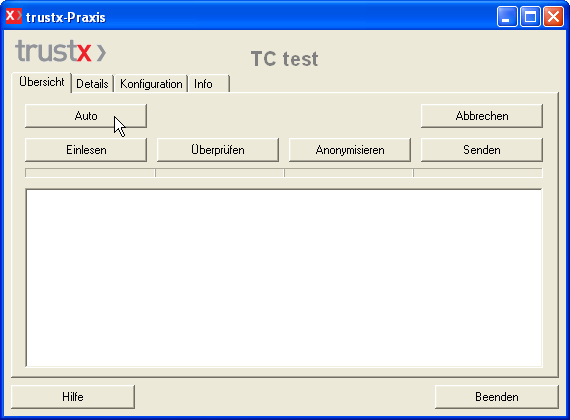
\includegraphics[width=0.8\textwidth]{abr15}\\
  \caption{TrustX-Programm}\label{fig:abr15}
\end{figure}

\subsubsection{Ausgabe in XML-Datei}
\begin{figure}
  % Requires \usepackage{graphicx}
  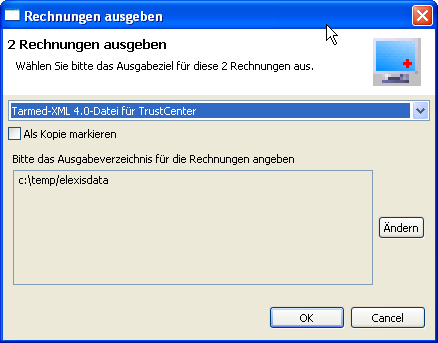
\includegraphics{abr16}\\
  \caption{Ausgabeziel XML}\label{fig:abr16}
\end{figure}

Dieses Ausgabeziel (Abb.\ref{fig:abr16}) speichert die gewählten Rechnungen in einem wählbaren Verzeichnis. Klicken Sie auf den 'ändern' - Button um das Verzeichnis zu ändern und dann auf OK um die ausgewählten Rechnungen dorthin zu schreiben. Dieses Format kann von einer Vielzahl von Intermediären weiterverarbeitet werden (Aerztekasse, Medidata, H-Clearing usw.). Deshalb ist dieses Ausgabeziel für alle Fälle geeignet, wo kein spezifisches Plugin existiert.

\section{Zahlungen verbuchen}

\subsection{Zahlungen manuell verbuchen}
\begin{figure}
  % Requires \usepackage{graphicx}
  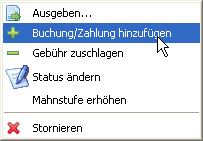
\includegraphics{abr17}\\
  \caption{Rechnungs-Menü}\label{fig:abr17}
\end{figure}
\begin{figure}
  % Requires \usepackage{graphicx}
  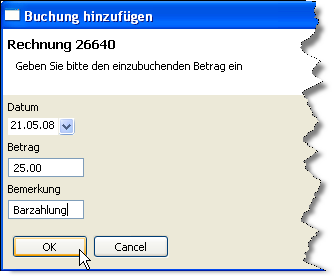
\includegraphics{abr18}\\
  \caption{Buchung hinzufügen}\label{fig:abr18}
\end{figure}

\index{Zahlungen!verbuchen}\index{Teilzahlung}\index{Barzahlung}
Wenn eine Teilzahlung oder eine Barzahlung, oder eine Zahlung über die 'normalen' roten Einzahlungsscheine hereinkommt, kann Elexis nicht von sich aus wissen, zu welcher Rechnung und welchem Patienten diese Zahlung gehört. In solchen Fällen müssen Sie die Zahlung manuell verbuchen. Klicken Sie dazu mit der rechten Maustaste auf die Rechnung, der die Buchung hinzugefügt werden soll (Abb.\ref{fig:abr17}. Es öffnet sich ein Dialog wie in Abb.\ref{fig:abr18}. Geben Sie dort das Buchungsdatum, einen Betrag in der Form x.xx und einen Buchungstext ein.


\subsection{ESR-Files einlesen}
\index{ESR}
Die Post oder Ihre Bank teilt Ihnen eine Methode mit, wie Sie die Dateien mit den Zahlungseingängen (ESR-Dateien) erhalten können. Meist geht das heutzutage über dasselbe Internet-Portal, das Sie auch zum e-Banking verwenden. Manchmal werden die Files aber auch auf Diskette oder per verschlüsselter Mail geschickt.
Diese Files enthalten sogenannte ESR-Records, anhand derer Elexis erkennen kann, zu welcher Rechnung eine Zahlung gehört.

\subsubsection{Die magische ESR-Zeile}
\label{esrline}
\begin{figure}
  % Requires \usepackage{graphicx}
  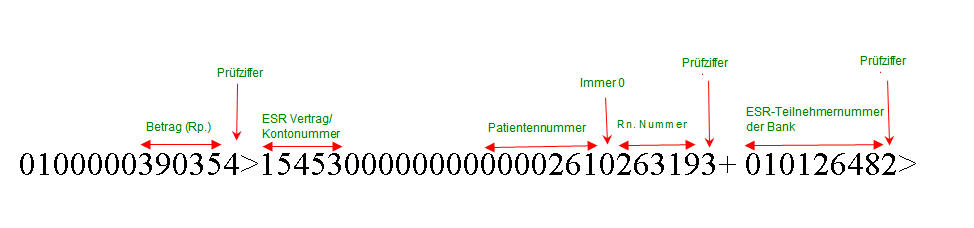
\includegraphics[width=1.0\textwidth]{abr19}\\
  \caption{BESR-Zeile}\label{fig:abr19}
\end{figure}

Eigentlich ist gar nichts Magisches dabei: Beim Drucken der Rechnung erstellt Elexis eine ESR-Zeile in von der Post festgelegtem Format, in die alle nötigen Angaben codiert sind, um die Zahlung aufs richtige Konto zu leiten und festzustellen, zu welcher Rechnung und welchem Patienten eine Zahlung gehört. Die ESR-Zeile sieht so aus wie in Abb.\ref{fig:abr19}. Bitte beachten Sie, dass Elexis hier nur Dinge eintragen kann, die Sie ihm mitgeteilt haben. Also wenn Sie beispielsweise keine ESR-Vertragsnummer für den betreffenden Mandanten eingegeben haben, dann wird da auch keine ESR-Vertragsnummer stehen können, sondern Elexis schreibt dann 'FEHLER'. Bei der \textbf{ZWINGEND vorgeschriebenen manuellen Kontrolle der ersten Rechnungen} sollte das auffallen.

\medskip

Die Bank schickt dann genau diese ESR-Zeile wieder mit, wenn eine Zahlung eingegangen ist, so dass Elexis sie 'wiedererkennt'. Speichern Sie also das von der Bank erhaltene ESR-File irgendwo ab, wo Sie es wiederfinden\footnote{Alle mir bekannten Banken geben dem ESR-File einen eindeutigen Namen, so dass nie mehrmals ein File mit demselben Namen kommt. Lassen Sie sich nicht verleiten, die Files unter immer demselben Namen zu speichern, sondern behalten Sie den Namen be  den die Bank dem File gibt. Elexis wird sich nämlich weigern, ein ESR-File mit einem Namen einzulesen, der schonmal eingelesen wurde, um Doppelbuchungen zu vermeiden. Falls Ihre Bank keine eindeutigen Dateinamen liefert, benennen Sie sie selbst um, dass sie eindeutig werden, z.B. 'ESR20080521.txt' (also jahr/monat/Tag im Namen eingebaut)} und öffnen Sie in Elexis die ESR-View (Abb.\ref{fig:abr20}).
\begin{figure}
  % Requires \usepackage{graphicx}
  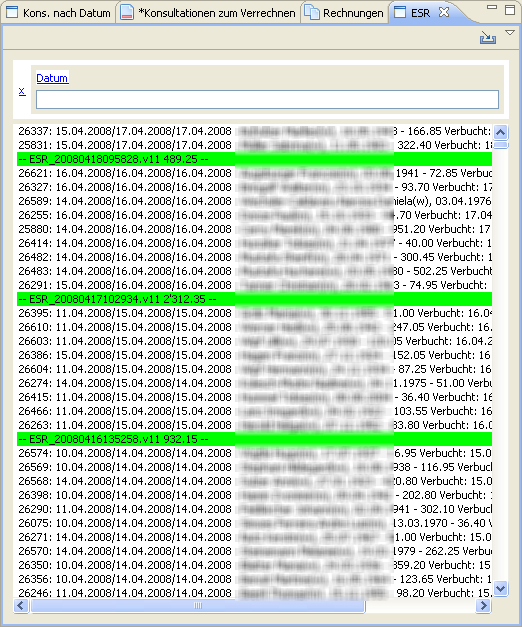
\includegraphics[width=0.9\textwidth]{abr20}\\
  \caption{ESR-View}\label{fig:abr20}
\end{figure}
\begin{figure}
  % Requires \usepackage{graphicx}
  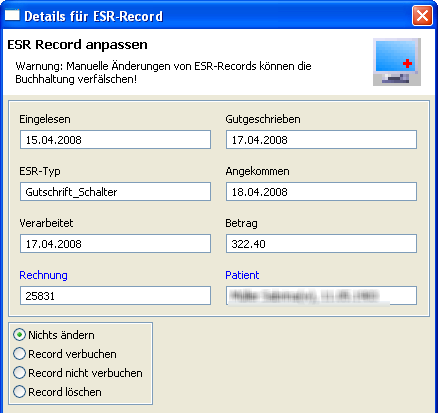
\includegraphics[width=0.9\textwidth]{abr21}\\
  \caption{ESR-Detail}\label{fig:abr21}
\end{figure}

Mit dem Import-Button können Sie das von Ihrer Bank erhaltene ESR-File importieren. Es erscheint dann jeweils ein grüner Balken, der eine Summe der in diesem File enthaltenen Zahlungen ausweist, und darüber die einzelnen ESR-Records. Wenn Sie einen ESR-Record näher ansehen wollen, können Sie darauf doppelklicken, dann erscheint ein Dialog wie in Abb.\ref{fig:abr21}.

\medskip

\index{Zahlungen!verbuchen}\index{Rechnung!Zahlungseingang}
Alle Records, die problemlos eingelesen und zugeordnet werden können, verbucht Elexis automatisch. Das heisst, die Zahlung wird der entsprechenden Rechnung gutgeschrieben und der Rechnungsstatus ggf. angepasst, z.B. von 'offen und gedruckt' auf 'teilweise bezahlt' oder 'bezahlt'. Wenn der bezahlte Betrag höher ist, als der noch offene Betrag der Rechnung fragt Elexis, ob es die Zahlung trotzdem verbuchen soll. Wenn Sie dann mit 'Ja' antworten, erhält die Rechnung den Status 'Zuviel bezahlt' und der offene Betrag bekommt einen negativen Wert. Wenn Sie mit 'Nein' antworten, wird die Zahlung nicht verbucht und wird in der ESR-Liste grau hinterlegt. Die Frage, was Sie damit machen sollen, kann Ihnen Elexis nicht beantworten, das müssen Sie dann selber entscheiden.

\medskip

Manchmal kann ein Record nicht zugeordet werden. Beispielsweise könnte ein Einzahler mit einem ebanking-Programm eine fehlerhafte ESR-Zeile eingegeben haben (Zwar gibt es eine Prüfziffer, um das zu verhindern, aber es können damit nicht alle Falscheingaben abgefangen werden). Oder es kann eine Zahlung sein, die von einer Rechnung eines anderen Programms stammt (welches natürlich andere Patienten- und Rechnungsnummern hat und die auch anders codiert). In diesem Fall entdeckt Elexis, dass z.B. die Rechnungsnummer gar nicht zum Patienten passt, oder dass Rechnungsnummer oder Patient gar nicht existieren. Solche ESR-Records können nicht verbucht werden, sondern erscheinen rot hinterlegt in der Liste.

\section{Mahnwesen}
Es soll schon vorgekommen sein, dass ein Patient die Rechnung nicht innerhalb der vorgegebenen Zahlungsfrist bezahlt hat. In solchen Fällen soll eine Zahlungserinnerung geschickt werden, bei weiterhin ausbleibender Zahlung dann eine zweite oder dritte Mahnung, und vielleicht soll der zusätzliche Aufwand mit einer Mahngebühr verrechnet werden. Es gibt zwei Möglichkeiten, dies anzugehen: manuell oder automatisch.

\subsection{manuelles Mahnen}
Ich selber bevorzuge diese Methode. Sie erlaubt mit, etwas feiner zu steuern, wann ich wen mahnen will. Die Frau X. hat immer bezahlt, der lasse ich es auch mal durchgehen, wenn sie diesmal drei Monate lang knapp bei Kasse ist, während der Herr Y. jeweils das Zahlen gern ganz vergisst, den mahne ich eher etwas früher.

\medskip

Am besten macht man das mit dem Filter der Rechnungsliste (Abb.\ref{fig:abr12}). Geben Sie dort unter 'Statusdatum von-bis' im bis-Feld ein Datum z.B. 40 Tage in der Vergangenheit ein, klicken Sie OK, wählen Sie im Status-Feld 'offen und gedruckt' und lesen Sie die Liste neu ein. Sie haben dann alle Rechnungen vor sich, die vor mehr als 40 Tagen gedruckt worden sind und seither keine Statusänderungen bekamen. Wenn Sie nun eine dieser Rechnungen Mahnen wollen, klicken Sie sie mit der rechten Maustaste an und wählen 'Mahnstufe erhöhen'. Diese Mahnung erhäkt dann den Status 'Zahlungserinnerung'. Beim nächsten Ausgeben wird sie den Status 'ZE gedruckt' erhalten.

\medskip

Machen Sie dasselbe, indem Sie ein Statusdatum z.B. 15 Tage in der Vergangenheit eingeben für den Status 'ZE gedruckt', dann erhalten Sie eine Liste aller Rechnungen, welche vor mehr als 15 Tagen den Status 'ZE gedruckt' erhalten haben und seither keine Statusänderung bekamen. Wenn Sie hier 'Mahnstufe erhöhen' eingeben, erhält die Rechnung den Status '2. Mahnung' und nach dem Drucken '2. Mahnung gedruckt'. Wenn Sie eine Mahngebühr hinzufügen wollen, dann klicken Sie die Rechnung nochmal mit der rechten Maustaste an, und wählen Sie 'Gebühr zuschlagen'. Es öffnet sich ein Dialog wie in Abb.\ref{fig:abr22}.
\index{Mahngebühr}
\begin{figure}
  % Requires \usepackage{graphicx}
  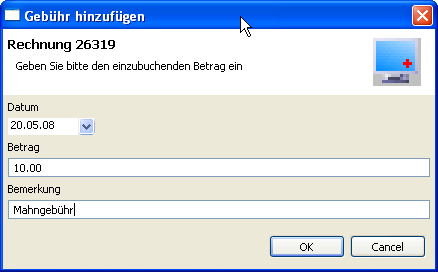
\includegraphics{abr22}\\
  \caption{Gebühr zuschlagen}\label{fig:abr22}
\end{figure}
Geben Sie dort das Datum, einen Betrag der Form x.xx und einen Text ein (Der Text wird so auf der Rechnung neben dem Betrag erscheinen).

\medskip
\index{Mahnung}\index{Betreiben}\index{Verlust}\index{Totalverlust}\index{Teilverlust}\index{Rechnung!abschreiben}
Gehen Sie analog für die Zweiten Mahnungen vor, um die Dritte Mahnung herauszulassen. Hier ist allerdings für Elexis Ende der Fahnenstange. Ob und wann Sie die Betreibung einleiten wollen, müssen Sie selber entscheiden und den Status selber auf 'In Betreibung' setzen. Alternativ können Sie den Status auf 'Teilverlust' oder 'Totalverlust' setzen, wenn Sie den offenen Betrag defintiv abschreiben wollen. (Sie können bei der Jahresbilanz dann die Verluste auflisten und in der Steuererklärung als Debitorenverluste angeben)

\medskip

Alle Rechnungen die noch auszugeben sind, können mit dem Pseudostatus 'zu drucken' aufgesucht werden. Diese Liste enthält dann also alle Rechnungen mit dem Status 'offen', 'Zahlungserinnerung', 'Zweite Mahnung' und 'Dritte Mahnung'. Nach der Ausgabe werden sie automatisch entsprechend auf 'offen und gedruckt', 'ZE gedruckt', '2. Mahnung gedruckt' und '3. Mahnung gedruckt' gesetzt.


\subsection{automatischer Mahnlauf}
Im unteren Abschnitt der 'Rechnungen'-View (\ref{fig:abr11}) ist Ihnen vermutlich bereits das Feld 'Mahnungen-Automatik' aufgefallen. Hier können Sie einstellen, nach wieviel Tagen jeweils die erste, zweite und dritte Mahnung erstellt werden soll (Tage jeweils von der letzten Statusänderung an gerechnet), und wieviel Mahngebühr zugeschlagen werden soll. Wenn Sie diese Angaben eingetragen haben, können Sie einen automatischen Mahnlauf mit dem 'Zauberstab' Button starten. Es werden dann automatisch erste, zweite und dritte Mahnungen erstellt und als 'zu drucken' zur Ausgabe bereitgehalten.

\section{Fehlerhafte Rechnungen}
\index{Rechnung!korrigieren}\index{Rechnung!löschen}
Let's face it: Manchmal enthält eine Rechnung Fehler. Wir haben nach bestem Wissen und Gewissen abgerechnet, aber der unbestechliche Krankenkassencomputer hat doch festgestellt, dass wir irgendwo 65 Rappen zuviel berechnet haben, und hat ein automatisches Schreiben (selbstverständlich per A-Post und mit Kopie an den Patienten) rausgelassen, in dem wir des Betrugs bezichtigt werden. Wir müssen also die Rechnung korrigieren und nach Canossa tragen. Bei letzterem kann Elexis auch nicht helfen, für die Korrektur aber gilt:

\medskip

\textit{Eine einmal erstellte Rechnung kann nicht geändert werden!}

\medskip

Der Grund dafür ist: Sobald Rechnungen korrigierbar wären, käme es mit Sicherheit vor, dass früher oder später unterschiedliche Rechnungen mit derselben Nummer im Umlauf wären. Wenn dann jemand (und sei es das Steueramt) eine Frage zu Rechnung 32456 hat, wird es schwierig zu sagen, welche Variante dieser Rechnung denn nun gemeint ist. Deshalb: \textit{Rechnungen sind unveränderlich}.

Das einzige, was man mit einer fehlerhaften Rechnung machen kann ist: Stornieren. Damit bleibt sie bestehen, aber es wird deutlich, das sie ungültig ist.

\medskip

\index{Rechnung!stornieren}
Um eine Rechnung zu stornieren, klicken Sie sie mit der rechten Maustaste an und wählen 'Stornieren'\footnote{Bitte stornieren Sie \textbf{nicht, niemals, gar nie} durch manuelle Änderung des Rechnungsstatus auf 'storniert', weil sonst die Buchungen nicht mehr stimmen}. Dadurch geschieht folgendes: Auf das Konto des Patienten wird eine Negativbuchung in Höhe des Rechnungsbetrags gemacht, und die Storno-Meldung wird an alle Ausgabeziele weitergegeben (Also wenn Sie die ursprüngliche Rechnung ans TrustCenter geschickt hatten, wird auch die Stornobuchung ans Trustcenter gemeldet).

Ausserdem können Sie angeben, ob Sie die Konsultationen für eine neue Verrechnung freigeben wollen (was üblicherweise der Fall ist) oder nicht - dann sind die entsprechenden Umsätze auf Nimmerwiedersehen verloren.

\medskip

Nach dem Storno sind die Konsultationen wieder offen, Sie können also alle nötigen Korrekturen anbringen und dann eine neue Rechnung erstellen.

\section{Patientenkonto}
\begin{figure}
  % Requires \usepackage{graphicx}
  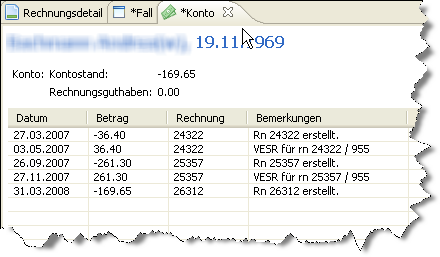
\includegraphics{abr23}\\
  \caption{Konto-View}\label{fig:abr23}
\end{figure}

Die oft auch interessante Frage, 'Wo stehe ich finanziell mit diesem Patienten' beantwortet die View 'Konto' (Abb.\ref{fig:abr23}). Hier sehen Sie alle Buchungen zum aktuell ausgewählten Patienten und das resultierende Guthaben resp. die resultierend Schuld.


\section{Merksätze}
\begin{itemize}
\item \textbf{WICHTIG: Beim ersten Mal und jedesmal wenn irgendetwas an der Konfiguration geändert wird, müssen die mindestens ersten paar Rechnungen von Hand kontrolliert werden. Stimmt der Taxpunkt? Stimmt die ESR-Zeile? Stimmt der Zahlungsempfänger? Stimmt die Kontonummer? usw.}
\item Eine Konsultation gehört immer zu genau einem Fall und genau einem Mandanten
\item Ein Fall gehört immer zu genau einem bestimmten Abrechnungssystem
\item Ein Fall ist unveränderlich wie ein Krankenkassenkärtli. Wenn etwas geändert werden muss, muss ein neuer Fall erstellt werden
\item Ein Fall kann Konsultationen mehrerer Mandanten beinhalten.
\item Eine Rechnung gehört immer zu genau einem Fall und genau einem Mandanten. Wenn ein Patient mehrere offene Fälle und/oder mehrere behandelnde Mandanten hat, wird für jeden Fall und jeden Mandanten eine separate Rechnung erstellt.
\item Eine einmal erstellte Rechnung ist unveränderlich. Sie kann nur storniert und neu erstellt werden.
\item Von der Bank heruntergeladene ESR-Dateien müssen \textbf{sofort} in Elexis eingelesen und verbucht werden, damit keine Zahlungseingänge verlorengehen.
\item \textbf{WICHTIG: Beim ersten Mal und jedesmal wenn irgendetwas an der Konfiguration geändert wird, müssen mindestens die ersten paar Rechnungen von Hand kontrolliert werden. Stimmt der Taxpunkt? Stimmt die ESR-Zeile? Stimmt der Zahlungsempfänger? Stimmt die Kontonummer? usw.}

\end{itemize}

\section{Informationen zu den einzelnen Tarifen}
\subsection{Tarmed}
In der Schweiz müssen Rechnungen gemäss Krankenversicherungsgesetz (KVG), Unfallversicherungsgesetz (UVG), Invalidenversicherungsgesetz (IV) und Militärversicherungsgesetz (MV) zwingend nach Tarmed abgerechnet werden.  Dem für alle Gesetze gleichen Leistungscodesystem stehen aber unterschiedliche Taxpunktwerte je nach Gesetz, Leistungserbringer und Kanton entgegen. Es müssen daher für KVG, UVG, IV und MV unterschiedliche Abrechnungssysteme erstellt werden, denen jeweils die am Ort der Leistungserbringung für dieses Gesetz gültigen Taxpunktwerte zugeordnet werden.  Ausserdem sollten je nach Gesetz und Abrechnungssystem auch folgende 'Notwendige Daten' (S. Abb. \ref{fig:abr2}) angegeben werden:\\

\begin{itemize}
\item \textbf{Generell}\begin{description}
\item [Kostenträger (Kontakt):] Die Stelle, welche die Rechnung letztlich zahlt. Ist bei Tiers Payant identisch zum Rechnungsempfänger, bei Tiers Garant nicht.
\item [Gesetz: (Text)]  Das bei der Rechnungserstellung anzuwendende Gesetz. Dies muss nur eingetragen werden, falls das Abrechnungssystem nicht gleich heisst, wie das Gesetz. Also wenn Sie z.B. ein Abrechnungssystem 'Konsilien nach KVG' haben, dann sollten Sie diesem Abrechnungssystem die Fallkonstante Gesetz=KVG zuordnen, wenn Ihr Abreczhnungssystem dagegen 'KVG' heisst, ist diese Konstante nicht nötig.
\item [Intermediär (Text):] Falls elektronisch übermittelte Rechnungen nicht direkt, sondern über einen Intermediär wie Ärztekasse, H-Clearing, mediserv etc. gesendet werden sollen, ist hier die EAN des Intermediärs anzugeben.
\end{description}
\item\textbf{KVG}\begin{description}
\item [Versicherungsnummer: ] Die Krankenkassen-Mitgliedsnummer des Patienten.
\end{description}

\item\textbf{UVG}\begin{description}
\item [Unfallnummer: ] Die vom Versicherer veregebene Unfallnummer.
\item [Unfalldatum: ] Nicht unbedingt identisch mit dem Fall-Beginndatum
\end{description}

\item\textbf{IV}\begin{description}
\item [AHV-Nummer: ] Die alte oder neue AHV-Nummer.
\item [Fallnummer: ] Die von der IV-Stelle vergebene Fallnummer
\end{description}

\end{itemize}

\subsubsection{medkey-RFE}
Im Jahr 2009 haben medkey und die Ärztekasse eine zusätzliche Codierung pro Konsultationsgrund entwickelt; den Konsultationsgrund oder neudeutsch RFE (Reason for Encounter). Die Kollision mit dem identischen Akronym aus dem ICPC-System war wohl unbeabsichtigt, sorgt aber gleichwohl für Verwirrung. Wir verwenden hier deshalb ausschliesslich den Begriff \textit{medkey-RFE}. Wenn Sie nicht an einem TrustCenter angeschlosen sind, brauchen Sie diesen Abschnitt nicht zu lesen, da ausser manchem TrustCentern niemand die medkey-RFE auswertet.

\medskip

Man erhofft sich von diesem Code eine bessere statistische Erfassung der Konsultationsgründe, was möglicherweise helfen könnte, Forderungen nach Taxpunktsenkungen im Rahmen der DRG-Einführung abzuwehren. Wenn Sie medkey-RFE verwenden wollen, brauchen Sie nur die View \textit{medkey-RFE} zu öffnen. Wenn Sie eine Konsultation ausgewählt haben oder bearbeiten, können Sie mit der linken Maustaste den Konsultationsgrund auswählen \footnote{Sie können auch, durch Klicken mit gedrückter STRG-Taste, mehrere Konsultationsgründe auswählen, aber medkey wird nur den am weitesten oben stehenden auswerten.}.

\medskip

Sie können in der medkey-RFE-View je nach persönlichen Vorlieben eine längere oder eine kürzere Anzeige der einzelnen medkey-RFEs einstellen. Ausserdem können Sie sich eine einfache Statistik über die von Ihnen  verwendeten medeky-RFEs anzeigen lassen (Vgl. Abb. \ref{fig:rfe1} - \ref{fig:rfe3}).

\begin{figure}[htbp]
     \begin{minipage}{0.32\textwidth}
      \centering
       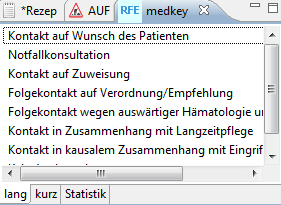
\includegraphics[width=0.95\textwidth]{rfe1}
       \caption{Lang}
       	\label{fig:rfe1}
     \end{minipage}\hfill
     \begin{minipage}{0.32\textwidth}
      \centering
       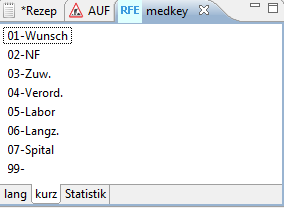
\includegraphics[width=0.95\textwidth]{rfe2}
       \caption{Kurz}
       \label{fig:rfe2}
     \end{minipage}
     \begin{minipage}{0.32\textwidth}
      \centering
       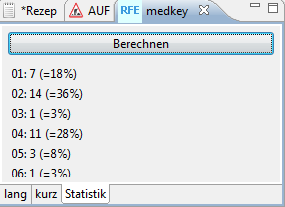
\includegraphics[width=0.95\textwidth]{rfe3}
       \caption{Statistik}
       \label{fig:rfe3}
     \end{minipage}
   \end{figure}

Beim Erstellen der Rechnung werden die medkey-RFE-Codes dann mit dem ersten Tarmed-Code der betreffenden Konsultation als 'remark' mitgeschickt. Das heisst auch: Sie können keine medkey-RFE übermitteln für eine Konsultation, die keine Tarmed-Positionen verrechnet hat.

\medskip

Auf der gedruckten Rechnung erscheint der medkey-RFE-Code nicht.

\subsection{Eidgenössische Analysenliste (EAL)}
Hier muss der Taxpunktwert unter \textsc{Datei-Einstellungen-Abrechnungssysteme-Labortarif} korrekt eingestellt werden.

\subsection{Physiotherapie}
\label{physiotarif}
\subsubsection{Abrechnungssystem}
\begin{figure}
  % Requires \usepackage{graphicx}
  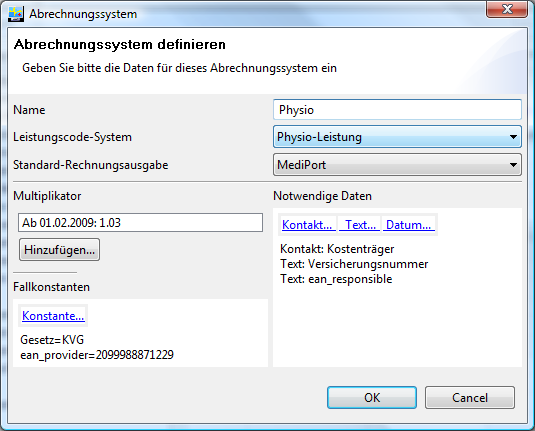
\includegraphics[width=0.95\textwidth]{abr25}\\
  \caption{Physio-Abrechnungssystem}\label{fig:abr25}
\end{figure}
Wenn Sie elektronisch abrechnen und der Empfänger Ihrer XML Rechnungen Wert auf die Angabe der ausführenden oder verantwortlichen Person\footnote{siehe auch \href{http://www.forum-datenaustausch.ch/mdinvoicerequest_xml4.00_v1.2_d.pdf}{XMLInvoice Referenzhandbuch Arzt-Rechnung}, Seite 58} legt, dann können Sie optional ein entsprechendes Abrechnungssystem konfigurieren (siehe Abschnitt \ref{Abrechnungssysteme} auf Seite \pageref{Abrechnungssysteme})
. Dabei können Sie die beiden XML Felder (ean\_provider, ean\_responsible) sowohl als Fallkonstante oder bei den Notwendigen Daten erfassen. Der Unterschied liegt darin, dass Fallkonstante automatisch in die Rechnung übernommen werden und die Notwendigen Daten pro Fall individuell erfasst werden müssen. Das Beispiel in Abb.\ref{fig:abr25} führt also die ausführende Person als Fallkonstante und die verantwortliche Person als Variable pro Fall.\linebreak
Hinweis: Beachten Sie, dass Fallkonstanten in der aktuellen Elexis Version 1.4.1 weder gelöscht, noch geändert werden können. Bei allfälligen Schreibfehlern müssen Sie das Abrechnungssystem löschen und neu erstellen.
\subsubsection{Stammdatenpflege}
Der Physiotarif kann in der Perspektive Leistungen bearbeitet werden (Abb.\ref{fig:abr26}). Die Leistungspositionen können dort manuell hinzugefügt und bearbeitet oder auch mittels Dreiecksmenü als CSV importiert werden (siehe \href{http://www.elexis.ch/jp/index.php?option=content&task=view&id=57}{Downloads Stammdaten auf www.elexis.ch}).
\begin{figure}
  % Requires \usepackage{graphicx}
  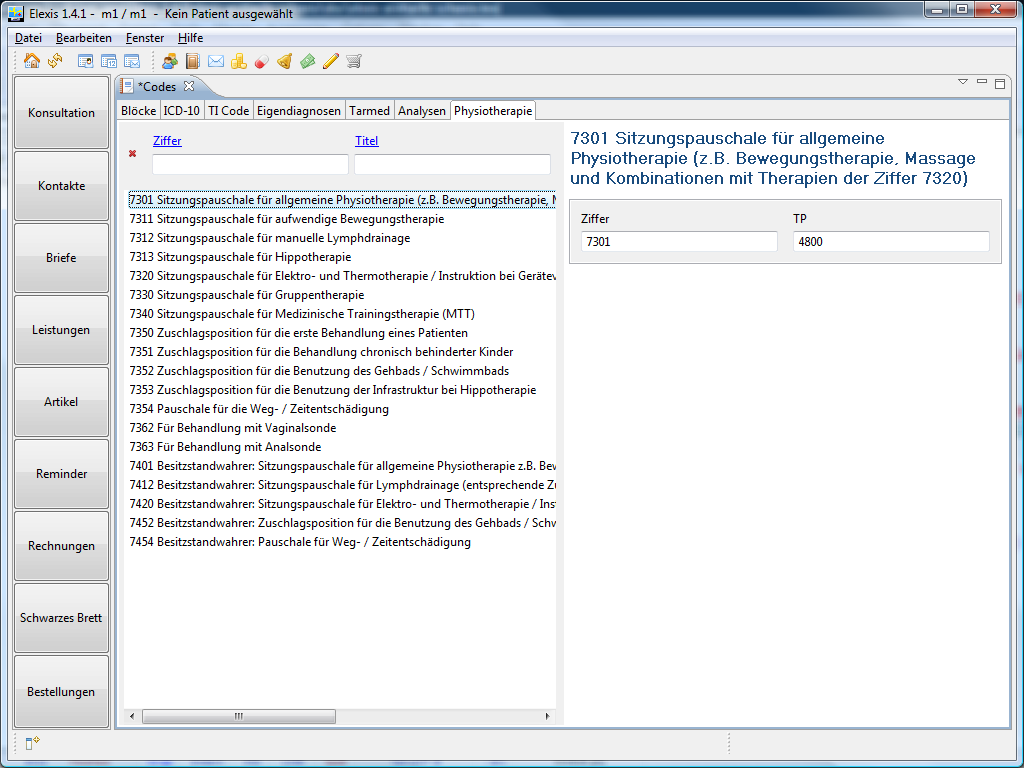
\includegraphics[width=0.95\textwidth]{abr26}\\
  \caption{Physio-Tarif Stammdaten}\label{fig:abr26}
\end{figure}
\subsubsection{Taxpunkte}
Damit die Behandlung der Taxpunkte in Elexis durchgängig gleich behandelt werden, erfolgt die Angabe der Anzahl Taxpunkte auch beim Physiotarif multipliziert mit 100. Für 24 Taxpunkte muss also 2400 eingegeben werden.
\subsubsection{Spezialpositionen}
Im Tarif sind nebst den herkömmlichen Leistungspositionen auch 2 Spezialfälle enthalten:
\begin{flushleft}
\begin{itemize}
\item
Fixpreispositionen:\linebreak
Bei den folgenden Positionen mutieren Sie bitte die Anzahl Taxpunkte so, dass bei der Multiplikation mit dem Multiplikator der gültige Frankenpreis resultiert. Aktuell gelten folgende Preise:\linebreak
7362 Für Behandlung mit Vaginalsonde: CHF 50.--\linebreak
7363 Für Behandlung mit Analsonde: CHF 90.--\linebreak
Beispiel:\linebreak
Multiplikator = 1.03\linebreak
TP für 7362 = 50/1.03 = 48.54\linebreak
Eingabe im Feld TP: 4854
\item Zuschlagsposition für Mittel und Gegenstände resp. Verbandsmaterial:\linebreak
Anstelle der Position 7360 aus dem Tarif verwenden Sie bitte die entsprechenden Artikel aus MiGeL
\end{itemize}
\end{flushleft}

\section{Weitere Unterstützung}
\subsection{Website}
Auf der Site http://www.elexis.ch werden aktuelle Informationen veröffentlicht. Es existiert auch eine Rubrik FAQ (Frequently Asked Questions), wo eventuell genau die Frage behandelt wird, die Sie auch grad stellen wollten. Schauen Sie also immer zuerst auf der Website nach. Diese enhält auch eine ausgezeichnete Suchfunktion, mit der Sie sowohl die ganze Site als auch nur die FAQ nach Stichwörtern durchsuchen können.

\subsection{Forum}
Unter http://www.elexis-forum.ch existiert ein Forum, in dem jede/r (auch Sie!) Fragen stellen und beantworten oder allgemeine Bemerkungen, Tips und Tricks, Kritiken usw. loswerden kann. Da Elexis ein community-Projekt sein will, wäre es schön, wenn Sie Fragen, die auf der Website nicht geklärt werden, im Forum besprechen würden, damit Andere auch etwas davon haben.
Wenn Sie sich als User im Forum angemeldet haben, dann können Sie es so einstellen, dass Ihnen automatisch nut die seit dem letzten Besuch neuen Themen angezeigt werden. Oder Sie können auch einen sog. RSS-Feed abonnieren, dann erhalten Sie jeweils die Titel der neuesten Beiträge als Newsfeed in Ihren Browser, ohne die Site aufsuchen zu müssen. Das Vorgehen, um Feeds zu abonnieren, ist in diesem Thread behandelt: http://www.elexis-forum.ch/viewtopic.php?t=10
Auch das Forum hat eine Suchfunktion, mit der Sie interessierende Themen nach Stichwörtern suchen können.

\subsection{Hilfe-Wiki}
Unter http://www.iatrix.org/pmwiki/pmwiki.php/Elexishilfe/Uebersicht existiert eine Hilfe-Seite, die ständig erweitert wird. Auch an dieser Seite können Sie aktiv mitmachen und eigene Erkenntnisse oder gelöste Probleme notieren, damit sie Anderen wieder zugute kommen.
Dieses Hilfe-Wiki wird standardmässig auch aufgerufen, wenn Sie von Elexis aus den 'Hilfe'-Button klicken, oder wenn Sie in irgendeiner View, zu der Sie Hilfe möchten, die F1-Taste drücken.

\subsection{Wartungsvertrag}
Wenn Sie einen Wartungsvertrag abgeschlossen haben, können Sie natürlich auch in diesem Rahmen Unterstützung erhalten. Über die genauen Bedingungen informiert Sie Ihr Elexis-Supporter.

\clearpage
\section{Index}
\printindex

\end{document}
